%%%%%%%%%%%%%%%%%%%%%%%%%%%%%%%%%%%%%%%%
% datoteka diploma-vzorec.tex
%
% vzorčna datoteka za pisanje diplomskega dela v formatu LaTeX
% na UL Fakulteti za računalništvo in informatiko
%
% vkup spravil Gašper Fijavž, december 2010
% 
%
%
% verzija 12. februar 2014 (besedilo teme, seznam kratic, popravki Gašper Fijavž)
% verzija 10. marec 2014 (redakcijski popravki Zoran Bosnić)
% verzija 11. marec 2014 (redakcijski popravki Gašper Fijavž)
% verzija 15. april 2014 (pdf/a 1b compliance, not really - just claiming, Damjan Cveta, Gašper Fijavž)

\documentclass[a4paper, 12pt]{book}

\usepackage[utf8x]{inputenc}   % omogoča uporabo slovenskih črk kodiranih v formatu UTF-8
\usepackage[slovene,english]{babel}    % naloži, med drugim, slovenske delilne vzorce
\usepackage[pdftex]{graphicx}  % omogoča vlaganje slik različnih formatov
\usepackage{fancyhdr}          % poskrbi, na primer, za glave strani
\usepackage{amssymb}           % dodatni simboli
\usepackage{amsmath}           % eqref, npr.
%\usepackage{hyperxmp}
\usepackage[pdftex, colorlinks=true,
						citecolor=black, filecolor=black, 
						linkcolor=black, urlcolor=black,
						pagebackref=false, 
						pdfproducer={LaTeX}, pdfcreator={LaTeX}, hidelinks]{hyperref}



%%%%%%%%%%%%%%%%%%%%%%%%%%%%%%%%%%%%%%%%
%	DIPLOMA INFO
%%%%%%%%%%%%%%%%%%%%%%%%%%%%%%%%%%%%%%%%
\newcommand{\ttitle}{Evalvacija čustev iz glasbe}
\newcommand{\ttitleEn}{Mood evaluation from music}
\newcommand{\tsubject}{\ttitle}
\newcommand{\tsubjectEn}{\ttitleEn}
\newcommand{\tauthor}{Primož Godec}
\newcommand{\tkeywords}{glasba, razpoloženje, evalvacija}
\newcommand{\tkeywordsEn}{music, mood, evaluation}



\usepackage{hyperref}
%%%%%%%%%%%%%%%%%%%%%%%%%%%%%%%%%%%%%%%%
%	HYPERREF SETUP
%%%%%%%%%%%%%%%%%%%%%%%%%%%%%%%%%%%%%%%%
\hypersetup{pdftitle={\ttitle}}
\hypersetup{pdfsubject=\ttitleEn}
\hypersetup{pdfauthor={\tauthor, p.godec9@gmail.com}}
\hypersetup{pdfkeywords=\tkeywordsEn}


 


%%%%%%%%%%%%%%%%%%%%%%%%%%%%%%%%%%%%%%%%
% postavitev strani
%%%%%%%%%%%%%%%%%%%%%%%%%%%%%%%%%%%%%%%%  
\renewcommand{\baselinestretch}{1.3} % ustrezen razmik med vrsticami
\setlength{\headheight}{15pt}        % potreben prostor na vrhu
\renewcommand{\chaptermark}[1]%
{\markboth{\MakeUppercase{\thechapter.\ #1}}{}} \renewcommand{\sectionmark}[1]%
{\markright{\MakeUppercase{\thesection.\ #1}}} \renewcommand{\headrulewidth}{0.5pt} \renewcommand{\footrulewidth}{0pt}
\fancyhf{}
\fancyhead[LE,RO]{\sl \thepage} \fancyhead[LO]{\sl \rightmark} \fancyhead[RE]{\sl \leftmark}



\newcommand{\BibTeX}{{\sc Bib}\TeX}

%%%%%%%%%%%%%%%%%%%%%%%%%%%%%%%%%%%%%%%%
% naslovi
%%%%%%%%%%%%%%%%%%%%%%%%%%%%%%%%%%%%%%%%  


\newcommand{\autfont}{\Large}
\newcommand{\titfont}{\LARGE\bf}
\newcommand{\clearemptydoublepage}{\newpage{\pagestyle{empty}\cleardoublepage}}
\setcounter{tocdepth}{1}	      % globina kazala

%%%%%%%%%%%%%%%%%%%%%%%%%%%%%%%%%%%%%%%%
% konstrukti
%%%%%%%%%%%%%%%%%%%%%%%%%%%%%%%%%%%%%%%%  
\newtheorem{izrek}{Izrek}[chapter]
\newtheorem{trditev}{Trditev}[izrek]
\newenvironment{dokaz}{\emph{Dokaz.}\ }{\hspace{\fill}{$\Box$}}

%%%%%%%%%%%%%%%%%%%%%%%%%%%%%%%%%%%%%%%%%%%%%%%%%%%%%%%%%%%%%%%%%%%%%%%%%%%%%%%
%% PDF-A
%%%%%%%%%%%%%%%%%%%%%%%%%%%%%%%%%%%%%%%%%%%%%%%%%%%%%%%%%%%%%%%%%%%%%%%%%%%%%%%

%%%%%%%%%%%%%%%%%%%%%%%%%%%%%%%%%%%%%%%% 
% define medatata
%%%%%%%%%%%%%%%%%%%%%%%%%%%%%%%%%%%%%%%% 
\def\Title{\ttitle}
\def\Author{\tauthor, p.godec9@gmail.com}
\def\Subject{\ttitleEn}
\def\Keywords{\tkeywordsEn}

%%%%%%%%%%%%%%%%%%%%%%%%%%%%%%%%%%%%%%%% 
% \convertDate converts D:20080419103507+02'00' to 2008-04-19T10:35:07+02:00
%%%%%%%%%%%%%%%%%%%%%%%%%%%%%%%%%%%%%%%% 
\def\convertDate{%
    \getYear
}

{\catcode`\D=12
 \gdef\getYear D:#1#2#3#4{\edef\xYear{#1#2#3#4}\getMonth}
}
\def\getMonth#1#2{\edef\xMonth{#1#2}\getDay}
\def\getDay#1#2{\edef\xDay{#1#2}\getHour}
\def\getHour#1#2{\edef\xHour{#1#2}\getMin}
\def\getMin#1#2{\edef\xMin{#1#2}\getSec}
\def\getSec#1#2{\edef\xSec{#1#2}\getTZh}
\def\getTZh +#1#2{\edef\xTZh{#1#2}\getTZm}
\def\getTZm '#1#2'{%
    \edef\xTZm{#1#2}%
    \edef\convDate{\xYear-\xMonth-\xDay T\xHour:\xMin:\xSec+\xTZh:\xTZm}%
}

\expandafter\convertDate\pdfcreationdate 

%%%%%%%%%%%%%%%%%%%%%%%%%%%%%%%%%%%%%%%%
% get pdftex version string
%%%%%%%%%%%%%%%%%%%%%%%%%%%%%%%%%%%%%%%% 
\newcount\countA
\countA=\pdftexversion
\advance \countA by -100
\def\pdftexVersionStr{pdfTeX-1.\the\countA.\pdftexrevision}


%%%%%%%%%%%%%%%%%%%%%%%%%%%%%%%%%%%%%%%%
% XMP data
%%%%%%%%%%%%%%%%%%%%%%%%%%%%%%%%%%%%%%%%  
\usepackage{xmpincl}
\includexmp{pdfa-1b}

%%%%%%%%%%%%%%%%%%%%%%%%%%%%%%%%%%%%%%%%
% pdfInfo
%%%%%%%%%%%%%%%%%%%%%%%%%%%%%%%%%%%%%%%%  
\pdfinfo{%
    /Title    (\ttitle)
    /Author   (\tauthor, damjan@cvetan.si)
    /Subject  (\ttitleEn)
    /Keywords (\tkeywordsEn)
    /ModDate  (\pdfcreationdate)
    /Trapped  /False
}


%%%%%%%%%%%%%%%%%%%%%%%%%%%%%%%%%%%%%%%%%%%%%%%%%%%%%%%%%%%%%%%%%%%%%%%%%%%%%%%
%%%%%%%%%%%%%%%%%%%%%%%%%%%%%%%%%%%%%%%%%%%%%%%%%%%%%%%%%%%%%%%%%%%%%%%%%%%%%%%

\begin{document}
\selectlanguage{slovene}
\frontmatter
\setcounter{page}{1} %
\renewcommand{\thepage}{}       % preprecimo težave s številkami strani v kazalu

%%%%%%%%%%%%%%%%%%%%%%%%%%%%%%%%%%%%%%%%
%naslovnica
%%%%%%%%%%%%%%%%%%%%%%%%%%%%%%%%%%%%%%%%
 \thispagestyle{empty}%
   \begin{center}
    {\large\sc Univerza v Ljubljani\\%
      Fakulteta za računalništvo in informatiko}%
    \vskip 10em%
    {\autfont \tauthor\par}%
    {\titfont \ttitle \par}%
    {\vskip 2em \textsc{DIPLOMSKO DELO\\[2mm]
    UNIVERZITETNI ŠTUDIJSKI PROGRAM PRVE STOPNJE RAČUNALNIŠTVO IN INFORMATIKA}\par}%
    \vfill\null%
    {\large \textsc{Mentor}: doc.\ dr. Matija Marolt\par}%
   
    {\vskip 2em \large Ljubljana 2014 \par}%
\end{center}
% prazna stran
\clearemptydoublepage

%%%%%%%%%%%%%%%%%%%%%%%%%%%%%%%%%%%%%%%%
%copyright stran
\thispagestyle{empty}
\vspace*{8cm}
{\small \noindent
Rezultati diplomskega dela so intelektualna lastnina avtorja.
Za objavljanje ali izkoriščanje rezultatov di\-plom\-ske\-ga dela je potrebno pisno soglasje avtorja, Fakultete za ra\-ču\-nal\-niš\-tvo in
informatiko ter mentorja%
\footnote{}


\begin{center}
\mbox{}\vfill
\emph{Besedilo je oblikovano z urejevalnikom besedil \LaTeX.}
\end{center}
% prazna stran
\clearemptydoublepage

%%%%%%%%%%%%%%%%%%%%%%%%%%%%%%%%%%%%%%%%
% stran 3 med uvodnimi listi
\thispagestyle{empty}
\vspace*{4cm}

\noindent
Fakulteta za računalništvo in informatiko izdaja naslednjo nalogo:
\medskip
\begin{tabbing}
\hspace{32mm}\= \hspace{6cm} \= \kill




Tematika naloge:
\end{tabbing}
Besedilo teme diplomskega dela študent prepiše iz študijskega informacijskega sistema, kamor ga je vnesel mentor. V nekaj stavkih bo opisal, kaj pričakuje od kandidatovega diplomskega dela. Kaj so cilji, kakšne metode uporabiti, morda bo zapisal tudi ključno literaturo.
\vspace{15mm}






\vspace{2cm}

% prazna stran
\clearemptydoublepage

%%%%%%%%%%%%%%%%%%%%%%%%%%%%%%%%%%%%%%%%
% izjava o avtorstvu
\vspace*{1cm}
\begin{center}
{\Large \textbf{\sc Izjava o avtorstvu diplomskega dela}}
\end{center}

\vspace{1cm}
\noindent Spodaj podpisani Primož Godec,
z vpisno številko \textbf{63110452}, sem avtor  diplomskega dela z naslovom:

\vspace{0.5cm}
\emph{Evalvacija čustev iz glasbe}

\vspace{1.5cm}
\noindent S svojim podpisom zagotavljam, da:
\begin{itemize}
	\item sem diplomsko delo izdelal samostojno pod mentorstvom
		doc.\ dr.\ Matije Marolta,

	\item	so elektronska oblika diplomskega dela, naslov (slov., angl.), povzetek (slov., angl.) ter ključne besede (slov., angl.) identični s tiskano obliko diplomskega dela,
	\item soglašam z javno objavo elektronske oblike diplomskega dela na svetovnem spletu preko univerzitetnega spletnega arhiva.	
\end{itemize}

\vspace{1cm}
\noindent V Ljubljani, dne 11. januarja 2011 \hfill Podpis avtorja:

% prazna stran
\clearemptydoublepage

%%%%%%%%%%%%%%%%%%%%%%%%%%%%%%%%%%%%%%%%
% zahvala
\thispagestyle{empty}\mbox{}\vfill\null\it%
Želim se zahvaliti mentorju Matiji Maroltu, za pomoč in spodbujanje pri raziskovanju in izdelavi diplomskega dela. Prav tako se želim zahvaliti Matevžu Pesku, ki si je vedno vzel čas, ko sem ga potreboval in s spodbujanjem poskrbel, da je bilo diplomsko delo napisano hitreje, kot bi bilo drugače. Zahvalil bi se tudi ekipi s katero smo sodelovali na projektu raziskovanja razpoloženja in glasbe. Ekipo sestavljajo Matevž Pesek, Matija Marolt, Mojca Poredoš, Jože Guna, Gregor Strle, Emilija Stojmenova in Matevž Pogačnik. Nazadnje bi se zahvalil še družini in prijateljem, ki mi vedno stojijo ob strani. 
\rm\normalfont

% prazna stran
\clearemptydoublepage

%%%%%%%%%%%%%%%%%%%%%%%%%%%%%%%%%%%%%%%%
% posvetilo
%%%%%%%%%%%%%%%%%%%%%%%%%%%%%%%%%%%%%%%%
\thispagestyle{empty}\mbox{}{\vskip0.20\textheight}\mbox{}\hfill\begin{minipage}{0.55\textwidth}%
...
\normalfont\end{minipage}

% prazna stran
\clearemptydoublepage

%%%%%%%%%%%%%%%%%%%%%%%%%%%%%%%%%%%%%%%%
% kazalo
\def\thepage{}% preprecimo tezave s stevilkami strani v kazalu
\tableofcontents{}


% prazna stran
\clearemptydoublepage

%%%%%%%%%%%%%%%%%%%%%%%%%%%%%%%%%%%%%%%%
% seznam kratic
%%%%%%%%%%%%%%%%%%%%%%%%%%%%%%%%%%%%%%%%

\chapter*{Seznam uporabljenih kratic}

\begin{tabular}{l|l|l}
  
  {\bf SVM} & support vector machine & metoda podpornih vektorjev \\
  \dots & \dots & \dots \\
\end{tabular}



% prazna stran
\clearemptydoublepage

%%%%%%%%%%%%%%%%%%%%%%%%%%%%%%%%%%%%%%%%
% povzetek
%%%%%%%%%%%%%%%%%%%%%%%%%%%%%%%%%%%%%%%
\addcontentsline{toc}{chapter}{Povzetek}
\chapter*{Povzetek}
V vzorcu je predstavljen postopek priprave diplomskega dela z uporabo okolja \LaTeX. Vaš povzetek mo ra sicer vsebovati približno 100 besed, ta tukaj je odločno prekratek.
\bigskip

\noindent\textbf{Ključne besede:} \tkeywords.
% prazna stran
\clearemptydoublepage

%%%%%%%%%%%%%%%%%%%%%%%%%%%%%%%%%%%%%%%%
% abstract
\selectlanguage{english}
\addcontentsline{toc}{chapter}{Abstract}
\chapter*{Abstract}
This sample document presents an approach to typesetting your BSc thesis using \LaTeX. A proper abstract should contain around 100 words which makes this one way too short.
\bigskip

\noindent\textbf{Keywords:} \tkeywordsEn.
\selectlanguage{slovene}
% prazna stran
\clearemptydoublepage

%%%%%%%%%%%%%%%%%%%%%%%%%%%%%%%%%%%%%%%%
\mainmatter
\setcounter{page}{1}
\pagestyle{fancy}

%%%%%%%%%%%%%%%%%%%%%%%%%%%%%%%%%%%%%%%
% UVOD
%%%%%%%%%%%%%%%%%%%%%%%%%%%%%%%%%%%%%%%

\chapter{Uvod}


\chapter{Pregled področja}

Lahko bi rekli, da je glasba ena najstarejših in zelo pomembnih aktivnosti na svetu. Razširjena je praktično po celem svetu in poznajo jo še tako izlirana in od ostalega sveta odmaknjena plemena. Znano je, da glasba na svetu obstaja že vsaj 50 000 let. Prva glasba naj bi takrat izvajali na Afriških tleh. Nato se je skozi čas razvijala in postala eden najpomembnejših sestavnih delov človekovega življenja. \cite{wallin2001origins} \cite{krause2012great} O pomebnosti glasbe priča dejstvo, da jo lahko slišimo praktično na vsakem koraku. Poslušamo jo doma, na poti, ko nam je dolgčas ali ko se želimo razvedriti, poslušamo jo ko smo na kavi ali ko smo v trgovini. Ponekod z pravo iziro glabe vplivajo na člonekove odločitve. Na primer v raznih trgovinah in lokalih z glasbo privlačijo kupce. Vse to priča o pomembnem vplivu glasbe pri človeku.  

Glasba pomembno vpliva na človekaova čustva in razploženje. To moč ima predvsem zaradi tega, ker ima neposredno pot do čustev. Glasbo namreč doživljamo z notranjimi čuti, zato ni potrebne predhodne interpretacije, kot je potrebna pri razumevanju tiskane besede.  Znano je da različna glasba vzbudi različna čustva in ima moč da zbudi potlačena čustva. Na vzdušje vpliva razmerje med toni. Mol pričara bolj melanholično vzdušje. Dur pa ba bolj veselo. \cite{lenko2009pomen}

V nadaljevanju poglavja bom povedal še nekaj o področju imenovanem pridobivanje informacij iz glasbe (Music information retrieval - MIR). To področje je pomembno, saj je osnova za temo moje diplomske naloge. Povedal bom nekaj o povezavi med razpoloženjem in glasbo. Pregledal bom datasete, ki obstajajo trenutno na področju razpoloženja in glasbe. Za konec pa bom predstavil še algoritme za evalvacijo čustev iz glasbe. 

\section{Pridobivanje informacij iz glasbe}

Pridobivanje infrormacij iz glasbe (Music information retrieval - MIR) je interdisciplinarna zannost, ki povezuje predvsem muzikologijo in računalništvo. \cite{pesek2012prepoznavanje} Vključuje pa tudi vede kot so psihologija, akademski študij glasbe, procesiranje signalov, strojno učenje in mnoge ostale. To področje je dokaj novo in se trenutno res hitro širi. Kljub temu, da je področje novo, je postalo že zelo široko. Pojavljajo se velike razlike v načinu obdelave in uporabe podatkov. Prav tako so cilji raziskovalcev zelo različni.

Ključni namen področja je pridobiti infromacije iz glasbe in še bolj pomembno te informacije potem uporabiti v različnih sistemih. Trenutno se največ dela na naslednjih sistemih. 

\paragraph{Sistem za predlaganje glasbe (Music Recommendation System)}

V osnovi taki sistemi predlagajo glasbo na podlagi zgodovine poslušane glasbe s strani uporabnika. Trenutno obstaja veliko takih sistemov kot sta Pandora in Last.fm, ampak le redki uporabljajo informacije pridobljene z MIR za svoje delovanje. Namesto tega veliko sistemov uporablja informacije na podlagi primerjave med uporabniki. Naprimer sistem predlaga glasbo, ki so jo poslušali uporabniki s podobno zgodovino poslušanja. Drugi spetu uporabljajo oznake k določeni glasbi ali pa kakšen druge informacije, ki niso del MIR-a. Te oznake lahko dodajo ali uporabniki ali pa tudi experti. Pri sistemu Pandora glasbo označujejo strokovnjaki pri sistemu Last.fm pa uporabljajo oznake dodane s strani uporabnikov. Oznake, ki se uporabljajo so lahko različne od tega, da označijo zvrst glabe, lahko oznake opisuejo tudi razploženje, ali je pesem instrumental ali ali ima voka, je vokal ženski, moški in podobno. Od kar pa se je področje MIR zelo razširilo vedno več sistemov uporablja tudi te informacije za predlaganje glasbe. 
 
\paragraph{Ločevanje pesmi na več pasov in prepoznavanje inštrumentov}

Sistem za ločevanje pesmi zna pesem v kateri nastopa več instrumentov in vokali, razstaviti tako, da imamo posamezne pasove v pesmi ločene. Na primer lahko loči po inštrumentih. Da lahko loči posamezne pasove potrebuje sistem za prepovznavanje inštrumentov. Zaradi tega sta ta sistema tako tesno povezana med seboj. 

Na tem področju obstaja že kar nekaj sistemov. Ti sistemi se veliko uporabljajo pri ustvarjanju podlag za karaoke. Tam je naprimer potrebno pesmi odvzeti vokal. Uporabljajo se tudi za izključevanje posameznih inštrumetnov iz podlage. Ti sistemi pa seveda še niso popolni. Veliko je še prostora za izbolšave. Velik problem je v tem kako najbolje ločiti vokal od ostalih delov pesmi, ker si vokal z določenimi inštrumenti deli frekvence.

\paragraph{Avtomatično prepisovanje glasbe}

Ti sistemi delujejo tako, da glasbo iz posnetka pretvarjajo v simbolični zapis. Največ se to uporablja za prepisovanje glasbe v zapis MIDI. Taki sistemi vključujejo kar nekaj podsistemov: detekcijo pojavov (onset detection), ocenjevanje trajanja, identifikacijo instrumentov, prepoznavanje ritma in ostale. Sistemi, ki trenutno obstajajo še niso popolni. Predvsem nastane problem, ko je v pesmi veliko inštrumentov in več polifoničnih nivojev. 

\paragraph{Avtomatična kategorizacija glasbe}

To so sistemi, ki znajo razvrstiti glasbo v več prej definiranih skupin. Na prodročju MIR se raziskovalci trenutno ukvarjajo predvsez kategorizacijo po žanrih in glede na čustva v glasbi. Za obe dve temi MIREX (Music Information Retrieval Evaluation eXchange) organizira tekmovanje v kategorizaciji glasbe. Raziskovalic lahko oddajo svoj algoritem, ki ga potem pežnejo na MIREX-ovem datasetu. Za kategorizacijo se uporabljajo tehnike za strojno učenje, kot so SVM \cite{ben2010user}, regresija, različna drevesa in še ostale.

\paragraph{Generiranje glasbe}

Eden od ciljev raziskovalcev v MIR pa je tudi narediti dober sistem za avtomatično generiranje glasbe. Zaenkrat še ne obstaja sistem, ki bi samostojno zgenerial dobro pesem. V trenutnih sistemih je potrebno predvsem veliko ročnega prilagajanja. 

\section{Evalvacija čustev iz glasbe}

Eno od pomembnih področij v MIR je zagotovo evalvacija čustev iz glasbe s pomočjo računalniških algoritmov. Ti algoritmi v osnovi delujejo tako, da najprej iz zvočnega zapisa izračunajo določene opisnike. V naslednjem koraku je potrebno na podlagi že obstoječe podatkovne zbirke natrenirati algoritem. Nato pa lahko izvedemo klasifikacijo na večji zbirki zvočnih posnetkov. Za delovanje teh algoritmo potrebujemo podatkovno zbirko z že obstoječimi podatki. Zato bom v naslednjem podpoglavju opisal kaj na tem področju že obstaja. Poleg tega bom naredil še pregled algoritmov, ki že obstajajo.

\subsection{Podatkovne zbirke}

Na področju razpoloženja v MIR obstaja že kar nekaj podatkovnih zbirk, ki vsebujejo različne oznake za glasbo. 

\paragraph{Podatkovna zbirka s filmsko glasbo}

Eerola et. al \cite{eerola2010comparison} so zbrali podatkovno zbirko, ki vključuje filmsko glasbo iz različnih znanih filmov. Ta podatkovna zbirka je razdeljena na dva dela. Prvi del vsebuje 361 glasbeni odlomkov. Za vsako odlomek imajo povprečno vrednost za prijetnost (ang. valence), aktivnost (ang. arousal) in  napetost (ang. tension). Poleg tega so za vsako pesem zbrali tudi oznake za čustva (vesel, žalosten, nežen in podbne). K vsaki odlomku je dodana tudi povprečna številčna vrednost o prisotnosti posameznega čustva izmed nabora čustev: jeza, strah, veselje, žalost in nežnost. Drugi del zbirke vsebuje 110 glasbenih odlomkov, ki so podmnožica odlomkov iz prvega dela. Poleg vseh oznak, ki jih ima prvi del ima ta del dodane še številčne vrednosti, ki označujejo prisotnost za čustvi lepota (beauty) in naklonjenost (liking). Ta podatkovna zbirka poleg podatkov vsebuje tudi glasbene odseke, ki so dlogi 15 sekund. Kar je dobro za evalvacijo podatkovne zbirke na različnih algoritmih. Poleg tega podatkovna zbirka vsebuje še podatke o naslovu filma za posamezen odlomek in podatek iz katerega dela pesmi je bil odrezan. 

\paragraph{Mood Swing Turk Dataset}

Podatkovna zbirka Mood Swing Turk Dataset \cite{schmidt2011modeling} je bila zbrana za 240 glasbenih odlomkov popularne glasbe. Za vsak odlomek vsebuje povprečno 17 vrednosti, ki opisujejo prijetnost (valence) in aktivnost (arousal). Dodani so še podatki o glasbi (naslov, avtor, album) in tudi podatki o poteku ocenjevanja (krog ocenjevanja v katerem so bile zbrane ocene in id uporabnika, ki je podal posamezno oceno). 

Sama podatkovna zbirka ne vsebuje uporabljenih glasbenih odsekov, so pa zaradi tega objavljene že izračunane značilnice za posamezno pesem. Podatkovna zbirka vsebuje naslednje zančilnice: Mel-frequency cepstral coefficients (MFCCs), Octave-Based Spectral Contrast, Statistical Spectrum Descriptors (SSDs), Chromagram in EchoNest Audio Features.

\paragraph{Cal500}

Podatkovna zbirka imenovana Cal500 \cite{turnbull2008semantic} ima zbrane podatek o razpoloženju za 500 pesmi. Pesmi so zbrane izmed zahodne popularne glasbe. Za vsako pesem ima oznako za razpoloženje (vesela, žalostna, jezna in podobne). V naboru imajo 18 možnih oznak. Podatkovna zbirka je bila anotirana ročno in ima 3 oznake na pesem. Poleg ročne anotacije so kaseneje anotirali tudi s pomočjo alogritma. Podatkovna zbirka vsebuje tudi glasbene datoteke.

\paragraph{MTV Music Dataset}

MTV Music Dataset \cite{schuller2010mister} vsebuje podatke za 192 pesmi izbrane iz MTV Europe Most Wanted lestvic med leti 1981 in 2000. Celotna podatkovna zbirka je bila anotirana s strni 5 ocenjevalcev. Vsaka ocena vsebuje vrednost za prijetnost (valence) in vrednost za aktivnost (arousal). Vsaka pesem je bila ozančena s strani 3h ocenejvalcev.

\paragraph{LAMP}

Podatkovna zbirka LAMP \cite{chu2010lamp} vsebuje podatke za 492 popularnih pesmi izdanih med 2002 in 2008. Podatkovna zbirka je bila labelirana s strani 400 anketirancev v treh korakih. V prvem je anketiranec dobil samo besedilo in  na podlagi tega določil prijetnost (valence) in aktivnost (arousal). V drugem koraku je dobil samo zvočni posnetek ter določal aktivnost in prijetnost. Isto je moral narediti v tretjem koraku na pdlagi besedila in zvočnega posnetka skupaj. 

\paragraph{Multi Modal}

Zadnja zbirka, ki jo bom opisal je tako imenovana Multi Modal \cite{panda2013multi} podatkovna zbirka. Vsebuje 903 posnetke, ki so tudi dodani podatkovni zbirki. Glasba je večinoma popularna zahodna. Za vsako pesem je določena ozanka s čustvom. Poleg tega pa je tudi vsaka pesem razvščena v enega od 5 razredov po razpoloženju. 

\subsection{Algoritmi za evalvacijo čustev iz glasbe} 

Vsi algoritmi za evalvacijo razpoloženja iz glasbe potrebujejo za svojo delovanje podatkovno zbirko, zato sem se v prejšnjem poglavju posvetil ravno tej temi. Poleg podtakov moramo poskrbeti tudi za različne značilke, na podlagi katerih se potem izvede klasifikacija. 

V osnovi lahko delovanje algoritmov za evalvacijo čustev iz glasbe razdelimo na dva dela. Prvi del je treniranje algoritma. V drugem delu pa algoritem dejansko izvede klasifikacijo. Prvi del (treniranje poteka tako), da uporabimo eno izmed mnogih metod (Support Vector Machine, regresijo, dreves ali kakšno drugo). Na podlagi značilnic in podatkov iz podatkovne zbirke (že določene končne vrednosti za glasbo) algoritem izračuna pravilo za preslikavo. Ta postopek se izvaja na delu podatkovne zbirke namenjene treniranju algoritma. Ko algoritem ve pravilo lahko izvedemo drugi del klasifikacije. Na podlagi značilnic in pravila za preslikavo sedaj algoritem določi vrednosti. Vrednost je lahko skupina po razpoloženju v katero uvorstimo določeno pesem ali pa številčna vrednost, ko določamo le prijetnost in aktivnost. Drugi del se izvede na drugem delu zbirke pesmi. 

To je opis splošnega delovanja algoritmov, ki je skupno vsem. Vsak od algoritmov pa ima svoje posebnosti. Zbral sem nekaj že obstoječih algoritmov, ki jih bom sedaj opisal.

Schmidt et. al \cite{schmidt2009projection} so uporabili regresijski algoritem (metoda najmanjših kvadratov) za klasifikacijo. Podatkovno zbirko so razdelili na dva dela tako, da so 70\% podatkovne zbirke uporabili za treniranje algoritma in 30\% za testiranje. Za značilke so uporabili Mel-frequency cepstrum in Chromo. Algoritem npoveduje prijetnost (valence) in aktivnost (arousal) pesmi. Parametra algoritem napoveduje ločeno. 

Panda et al. \cite{panda2013multi} so uporabili več algoritmov za napovedovanje in primerjali točnost napovedovanja. Uporabili so: Support Vector Machines, K-nearest Neighbours, C4.5 in Naive Bayes. Algoritem je izvaja klasifikacijo na podlagi 19 značilnic izračunanih iz glasbenega posnetka. Tem značilnicam so dodali tudi značilinice pridobljene iz MIDI signala in značilnice iz besedil. Izvajal je klasifikacijo v 5 gruč, ki so definirane za MIREX tekmovanje (tabela \ref{mirextask}).  Kot najboljši algoritem se je izkazal SVM. Samo na podlagi značilnic iz zvočnega zapisa je dosegel natančnost 64\%. Ko so dodali še značinice iz MIDI zapisa in besedil, pa se je natančnost zmanjšala na 61.1\%. Algoritem so preizkusili na podatkovni zbirki z 903 pesmimi. 

Laurier et. al \cite{laurier2007audio} so za evalvacijo uporabili Support Vector Machine (SVM) \cite{ben2010user}. Algoritem za delovanje uporablja 133 značilk. Tudi ta algoritem deluje tako, da kot rezultat za vsako pesem vrne eno od petih gurč opisanih v tabeli \ref{mirextask}. Preizkusili so več različnih SVM metod in ugotovili, da najboljše rezultate vrača metoda C-SVC z RBF (Radial Basis Function) jedrom iz SVMlib knjižnice. 

Diane Watson \cite{watson2012modeling} je uporabila klasifikator z Bayesovimi mrežami in Markove ocene. Kot rezultat je algoritem napovedoval prijetnost (valence) in aktivnost (arousal). Za razliko od ostlih je ona uporabila podatke, ki niso bili zajeti v laboratorijskem okolju ampak v vsakdanjem življenju. Uporabniki so skladbe ocenjevali s pomočjo pametnih telefonov kjerkoli so se nahajali v trenutku, ko jih je aplikacija prosila za oceno. Poleg značilnic iz glasbe je algoritem upošteval tudi podatke o tem kako prijetno se uporabnik počuti v času ocenjevanja in podatke o njegovi aktivnosti ter še nekatere druge podatke o stanju in okolju med tem ko je ocenjeval. Algoritem je dosegel natančnost 67\% za aktivnost (arousal) in 75\% za prijetnost (valence). 

Sari et. al \cite{saari2013role} so uporabili Semantic Layer Projection (SLP) metodo za klasifikacijo. Za klasifikacijo so uporabili značilnice, končni rezultat pa so oznake s čustvi. Za razliko od prej opisnih metod, ki preslikavo izvedejo v enem koraku je tu drugače. Tukaj najprej preslikajo značilnice v tri dimenzionalni prostor z uporabo metode delnih najmanjših kvadratov (Partial Least Squares - PLS) in potem v drugem koraku na podlagi teh vrednosti določijo razpoloženje. Naj omenim, da so poskusili tudi algoritem v kombinaciji z tekstovnimi oznakami, vendar je deloval slabše. 


\begin{table}[htb]
	\caption{Gruče z čustvi, ki se uporabljajo v MIREX mood tekmovanju}
    \begin{tabular}{|l|l|}
    \hline
    Gruče   & Čustva  \\
    \hline                                                      
    Gruča 1 & passionate, rousing, confident, boisterous, rowdy             \\
    Gruča 2 & rollicking, cheerful, fun, sweet, amiable/good natured        \\
    Gruča 3 & literate, poignant, wistful, bittersweet, autumnal, brooding  \\
    Gruča 4 & humorous, silly, campy, quirky, whimsical, witty, wry         \\
    Gruča 5 & aggressive, fiery, tense/anxious, intense, volatile, visceral \\
    \hline
    \end{tabular} 
    \label{mirextask}   
\end{table}


\chapter{Naš dataset}

Tema moje diplomske naloge je vsekakor evalvacija čustev iz glasbe s pomočjo računalnikih algoritmov. Dobre evalvacije pa ni možno narediti brez dobrega dataseta, zato smo se odločili, da zgradimo svoj dataset, ki bo osnova za raziskovanje povezave med čustvi in glasbo. Poleg tega smo se odločili, da datset nadgradimo s podatki o barvah, ki po mnenju anketirancev najbolje odražajo posamezno skladbo. Tako smo s tem pridoli še povzavo med čustvi, glasbo in barvami.

V naslednjih delih bom predstavil, kako smo zbirali podatke iz našega dataseta. Kasneje pa bom še analiziral nekatere podatke iz našega dataseta.

\section{Zbiranje dataseta}

Dataset smo zbirali s spletno anketo, ki smo jo sami implementirali. Še preden pa smo lahko naredili glavno anketo, smo morali sprejeti še nekaj odločitev, kako zgraditi anketo, da bo dala dobre in predvsem uporabne rezultate. Prva stvar, kjer je bil potreben premislek, je izbor oznak za emocije. Ugotovili smo, da obstajajo nekatere osnovne oznake za čustva, ki si jih je možno pogledati v \cite{dalgleish1999handbook}, ni pa standardnega seta oznak, ki bi se uporabljal na področju povezanem z razpoloženjem in glasbo. Nekatri avtorji so izbrali zbirko oznak čisto ituitivno naprimer \cite{wu2013spectral}. Zaradi tega smo se odločili, da naredimo prliminarno raziskavo v obliki ankete. 

\subsection{Preliminarna analiza}

Kot omenjeno smo preliminarno analizo izvajali s pomočjo ankete. To smo izvedli v elektronski obliki. V njej smo želeli preveriti osnovno strukturo glavne ankete, primernost elementov ankete in najbolj pomembno ugotoviti, katere oznake za čustva, so tista, ki bojo uporabljena v glavni anketi. Čustva smo izbirali tako, da je moral uporabnik za 46 oznak povedati, kako je neko čustvo prisotno pri njemu v tistem trenutku. Uporabnik je to označil na skali od 1 do 7. Iz tega seznama je bilo potem izbranih 17 osnovnih oznak uporabljenih v glavni anketi: aktivno, budno, dremavo, neaktivno, nesrečno, nezadovoljno, razočarano, sproščeno, srečno, utrujeno, vedro, veselo, zadovoljno, zaspano, žalostno, mirno in jezno.

slika skale

Kot sem že omenil nas je zanimala tudi struktura vprašalnika, ki je ostala približno enaka s to razliko, da smo v novem vprašalniku dodali del z glasbnenimi odseki ampak več o tem v [ref na chapter].

Poleg tega pa smo testirali tudi elemente uporabljene v anketi (7 stopenjska skala, neskončni barvni krog, izbira z radio gumbi in tekstovnimi polji). Ugotovili smo, da moramo nekatere elemente spremeniti. Najbolje smo spremenili barvno skalo, saj smo jo omejili na barvni krog z 49 možnostmi izbire. To je bilo potrebno, ker je imel na naeskončni skali uporabniki preveliko možnost izbiranja, obenem pa je bil sistem trodimenzionalen, kar večina uporabnikov sploh ni opazila in so nastavljali samo odtenek na svetlost pa so pozabili. Skala z 49 možnostmi (prikazana na sliki \ref{colorwheels}) se je izkazala kot odlična alternativa, saj še vedno ponuja veliko možnosti izbire barv, je prijazna uporabniku in pridobljeni podatki so boljši.

Poleg zamenjave barvnega kroga smo zamenjali tudi nekaj ostalih elementov. V delu, kjer uporabnik ozanči tri svoje najljubše žanre smo se odločili, da namesto vpisnih polj uporabniku ponudimo, da iz seznama izbere in na drug seznam potegne svojo izbiro. Za to smo se odločili, ker so uporabniki tja vpisovali tudi žanre, ki niso osnovni in tisti, ki sploh niso žanri. Prav tako nam je ta preliminarni vprašalnik pomagal izbrati kateri žanri so tisti, ki jih bomo uporabniku ponudili. Zamenjali smo še način, kako uporabnik vnese svoje trenutno razpoloženje in za ta namen uporabili nov element MoodGraph, ki ga bom opisal kasneje. 

\begin{figure}[ht]
\centering
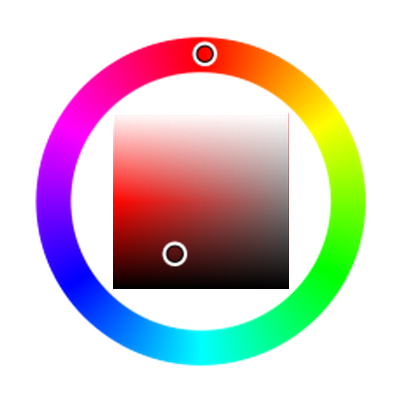
\includegraphics[width=60mm]{colorwheelold.png}
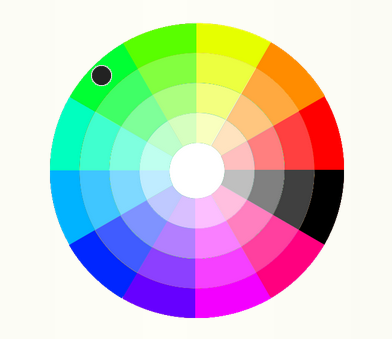
\includegraphics[width=60mm]{colorwheel.png}

\caption{Prvi barni krog smo v preliminarni anketi. V zunanjem krogu je bilo možno izbrati odtenek (hue) v notranjem pa je bilo možno izbirati nasičenost in svetlost. Drugi krog smo uporabili v glavni anketi. Imel je možnost izbire med 49 barvami. Rezina predstavljajo en barvni odtenek, proti notranjosti pa se spreminaja svetlost in intenzivnost. }
\label{colorwheels}
\end{figure}

\subsection{Glavna anketa}

Ko so bile izbrane oznake in struktura v grobem določena smo se lotili implementacije druge verzije vprašalnika, ki predstavlja glavni vprašalnik za zbiranje naše podatkovne zbirke. 

Glavni vprašalnik je bil sestavljen iz treh delov. V prvem delu smo spraševali po uporabnikovih demografskih podatkih, o poslušanju glasbe in glasbeni izobrazbi. V drugem delu nas je zanimalo predvsem uporabnikova percepcija razpoloženja, glasbe in barv. V tretjem delu so morali uporabniki ozačiti razpoloženje in barve v odlomku glasbe. 

\paragraph{Prvi del}

V tem delu smo spraševali o anketirančevi starosti, spolu in o tem ali živi na podeželju ali v mestu. Uporabnika smo vprašali tudi o tem ali je pod vplivom drog ali substanc. Zanimali so nas tudi podatki o glasbeni izobrazbi in o tem ali udeleženec igra inštrument ali poje. Poleg tega nas je še koliko časa dnevno uporabnik posluša glasbo. Anketrianec je moral tudi izbrati do tri svoje najljubše žanre in jih razporediti po priljubljenosti. To smo zajemal s pomočjo elementa prikazanega na sliki \ref{genresel}, kjer je uporabnik izmed seta 20 žanrov izbral najljubše in jih potegnil potegnil v stolpec desno ter razporedil po priljubljenosti. 

\begin{figure}[h!t]
\centering
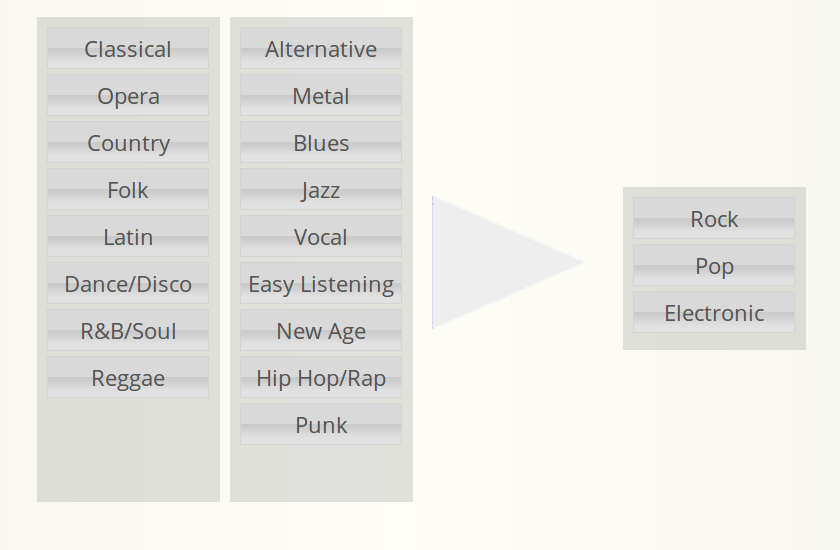
\includegraphics[width=10cm]{genresel.png}

\caption{Element v anketi uporabljen za izbiro najljubših žanrov}
\label{genresel}
\end{figure}

\paragraph{Drugi del}

Drugi del je namenjen zaznavanju anketirancovega trenutnega razpoloženja in njegove percepcije oznak za razpoloženje in barve za razpoloženje. To podatke zajemamo zato, ker na tak način lahko ugotovimo vzrok v različnih ocenah razpoloženja pri delu z glasbo. 

Na začetku je bil uporabnik vprašan kako bi svoje razpoloženje opisal s točko v prostoru, kjer zajemamo prijetnost in aktivnost (VA prostor) [ref]. To je dvodimenzionalen prostor, kjer na x osi od leve proti desni narašča prijetnost in od spodaj navzgor aktivnost.    Svoje razpoloženje je moral opisati tudi z izbiro barve s pomočjo elementa \ref{colorwheels}. 

Uporabnik je moral svoje razpoloženje opisati tudi z tem, da je povedal kako je posamezno čustvo pri nejm izraženo v trenutku reševanja ankete. To smo zajemali s pomočjo novega elementa imenovanega MoodStripe. Potrebno je bilo potegniti posamezne oznake čustev v prostor, kjer od leve proti desni narašča prisotnost posamznega čustva. Če je anketiranec postavil čustvo skrajno levo to pomeni, da to čustvo pri njem ni prisotno, če pa ga je posavil skrajno desno to pomeni, da je čustvo zelo prisotno 

\begin{figure}[ht]
\centering
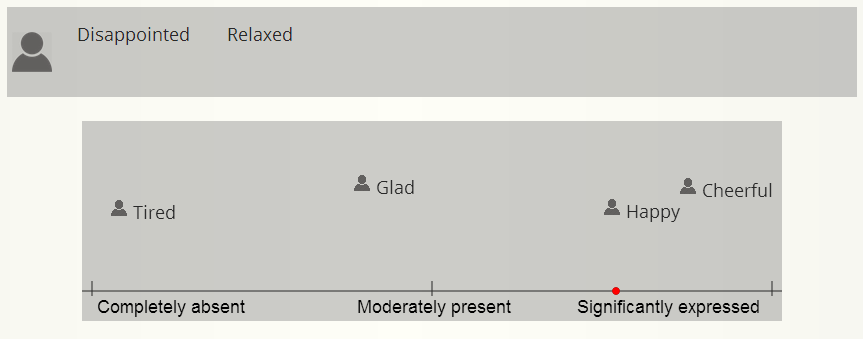
\includegraphics[width=10cm]{moodstripe.png}

\caption{Element za zajemanje pristnosti posameznega čustva imenovan moodstripe.}
\label{genresel}
\end{figure}

V drugem delu smo uporabnika povprašali tudi o njegovi percepciji posameznega čustva. Anketiranec je moral za vsako čustveno oznako povedati kako prijetno je to čustvo in kako aktivno je (VA vrednost). To smo zajemali s pomočjo elementa imenovanega enokategorni MoodGraph (slika \ref{moodgraph}). To je 2D prostor, kjer je na vodoravni osi prijetnost in na navpični osi anktivnost. Uporabnik je ozake čustev prikazane nad grafom potegnil v to ravnino na mesto za katerega misli, da ga najbolje opisuje. 

\begin{figure}[ht]
\centering
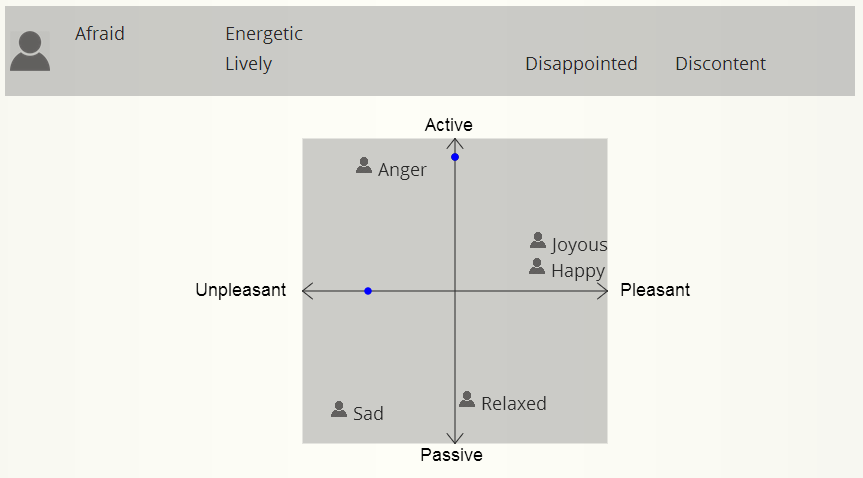
\includegraphics[width=10cm]{images/moodgraph.png}

\caption{}
\label{moodgraph}
\end{figure}

Poleg tega kako si uporabnik predstavlja posamezno čustvo v VA prostoru nas je zanimalo tudi kako bi uporabniku opisal ista čustva z barvno. To smo izvedli s pomočjo barvnega krogra (slika \ref{colorwheels}), ki sem ga že opisal zgoraj. 

\paragraph{Tretji del}

V tretjem delu smo vprašali anketirance, da ozačijo 10 glasbenih odlomkov dolgih 15 sekund. Odlomki so bili izbrani iz nabora 200 odlomkov. Glasba je bila izbrana tako, da je bila uporabnikom nepoznana. S tem smo se izognili pristranskosti zaradi uporabnikovega poznavanja določene glasbe in vpliva dogodkov, ki so se mu zgodili ob poslušanju določene pesmi. Vsak uporabnik je dobil samo 10 odlomkov iz tega razloga, da uporabnikov nebi preveč obremenili in bi zaradi tega dobili slabše ocene. 

Glasba je bila izbrana iz 4 različnih virov. 80 pesmi smo izbrali iz odprte podatkovne zbirke Jamendo. Iz tega vira smo izbrali bolj vsakdanjo glasbo različnih zvrsti. Naslednjih 80 pesmi smo vzeli iz zbirke filmske glasbe opisane v \cite{eerola2010comparison}. Dodali smo še 20 slovenskih etno pesmi in 20 pesmi iz nabora moderne elektro-akustične glasbe. 

Za vsak odlomek je moral uporanik narediti dve stvari. Najprej je s pomočjo barvnega kroga (slika \ref{colorwheels}) povedal s katero barvo bi opisal posamezno pesem. Nato pa je v drugem koraku izbral katera čustva so izražena v odlomku in katera čustva posamezna glasba vzbudi pri njem. Za prvo je izbiral izmed nabora 14 oznak, za drugo pa je iz nabora 10 ozank. Poleg tega, da je izbral posamezno oznako jo je moral še uvrstiti v VA prostor. S tem smo zajeli tudi podatek kako si predstavlaja določeno oznako pri posamezni pesmi. Naprimer pri neki pesmi je lahko veselje zelo aktivno, pri drugi pa majn. Poleg tega nam ta podatek da možnost, da raziskujemo tudi samo kako si uporabnik v VA prostoru predstavlja posamezno pesem. Za zajemanje tega podatka smo uporabili dvokategorni MoodGraph prikazan na sliki \ref{moodgraphdvo}.

\begin{figure}[hbt]
\centering
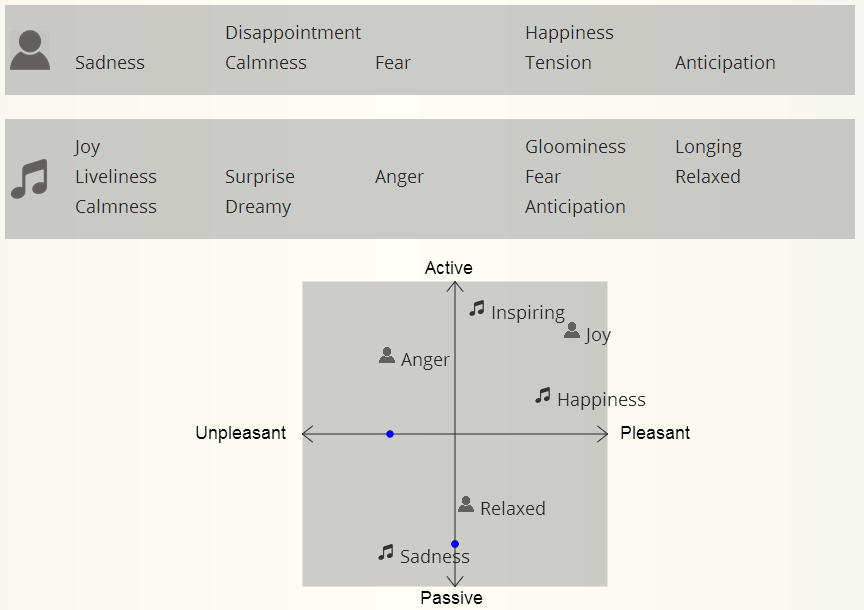
\includegraphics[width=10cm]{images/moodgraphdvo.png}

\caption{}
\label{moodgraphdvo}
\end{figure}

\subsection{Evaluacijska anketa}

\section{Sestava datasta}

Sedaj sem opisal kako smo zibrali podatke za podatkovno zbirko, nisem pa še povedal kakšni so ti podatki. Kot anketa so tudi podatki razdeljeni v tri dele. V prvem delu smo zbrali več kot 1400 odgovorov in s tem tudi toliko vpisov v naši zbirki. V drugem delu je vpisov malo več kot tisoč. V tretjem delu, kjer je moral uporabnik oceniti 10 pesmi pa smo zbrali več kot 7200 vpisov v podatkovno zbirko. Torej je ta del izpolnjevalo nekaj več kot 700 anketirancev.

V prvem delo so podatki, ki opisujejo anketirance. Za vsakega imamo podtek o starosti na leto natančno, o spolu in o tem ali živi na podeželju ali v mestu. Poleg tega smo zbrali podatke o tem koliko časa se ukvarja z glasbo in koliko časa je hodil v glasbeno šolo do leta natančno ter koliko časa na dan posluša glasbo. Tukaj je uporabnik poslušanje glabe uvrstil v eno od kategorij: do 1 ure, od 1 do 2 ure, od 2 do 3 ure in več kot 3 ure. Imamo tudi podatek o največ treh najljubših glazbenih zvrsteh, ki jih anketiranec najraje posluša. Tukaj je anketiranec podal najmanj eno in največ tri zvrsti. Zanimalo nas je še psihofizično stanje anketiranca med reševanjem. Torej imamo podatek ali jemlje zdravila, ki vplivajo na razploženje ter če je bil v trenutku reševanja pod vplivom drog ali alkohola. 

Drugi del podatkovne zbirke vsebuje podatke o anketirancevem razpoloženju v trenutku, ko je izpolnjeval anketo in o tem kako si anketiranec predstavlja posamezna čustva. Uporabnikono razploženje opisujejo trije podatki. Prvi je točka v VA prostoru (x in y koordinata). Drugo je barva v barvnem krogu (tukaj hranimo podatek o tem katero barvo je  anketiranec izbral). Tretji pa je vrednost kako močno je posamezno čustvo iza naobra 17 čustev, izraženo pri anketirancu v tistem trenutku. Hranimo vrednost med 0 in 1 za vsako čustvo. Kot sem že omenil drugi del vsebuje tudi podatek o tem kako si anketiranec predstavlja čustva. Za nabor 10 čustev imamo podatek kam v VA prostoru spada to čustvo po mnenju anketiranca in barvo s katero ga je anketiranec ozačil. 

Tretji del podatkovne zbirke je malo drugačen. Tu nimamo le enega odgovora na anketiranca ampak do 10 odgovorov. Za vsako pesem en odgovor. Imamo podatek o tem katera čustva so izražena v glasbi in katera so vzbujena pri anketirancu. Poleg tega pa imamo za vsakga od izbranih čustev še podatek kam v VA prostor ga bi anketiranec postavil. Za vsako pesem imamo še podatek o barvi s katero je anketiranec ozančil glasbeni odlomek.  

\section{Analiza podatkov}

\subsection{Demografska analiza}




\bibliography{diploma}{}
\bibliographystyle{plain}

\end{document}

